\documentclass[12pt,a4paper,faculty=ea,language=en,doctype=report]{ugent-doc}
\geometry{bottom=2.5cm,top=2.5cm,left=2.5cm,right=2.5cm} 
\renewcommand{\baselinestretch}{1.15}

\usepackage{fontspec}
\setmainfont[
  ItalicFont=SourceSerifPro-LightItalic.ttf
]{SourceSerifPro-Light.ttf}
\setsansfont{WorkSans-Regular.ttf}
\usepackage[english]{babel}
% \usepackage{libertine}
% \usepackage{libertinust1math}
\usepackage{amsmath} % math equations

% code snippets
\setmonofont[
  ItalicFont=SourceCodePro-Italic.ttf,
  BoldFont=SourceCodePro-SemiBold.ttf,
]{SourceCodePro-Regular.ttf}
\usepackage{listings}

% transcriptions:
\usepackage{xparse}
\usepackage{enumitem}

% acronyms
\usepackage[printonlyused,withpage]{acronym}

% figures
\usepackage{graphicx} 
\usepackage{changepage}
\usepackage{pgfplots}
\graphicspath{{./figures/}}

% Bibliography
\usepackage[backend=biber, style=apa, sorting=nyt, hyperref=true]{biblatex} 
\addbibresource{references.bib}
\usepackage{csquotes} % Suggested when using babel+biblatex

% Ugent specific
\usepackage[colorlinks=true, allcolors=ugentblue]{hyperref} % Hyperreferences
\usepackage[parfill]{parskip} % Whitespace between paragraphs and no indentation

% code snippets
\usepackage{listings}
\usepackage{minted}
\usepackage{caption}
\captionsetup{justification=centering, margin=2cm}
\definecolor{mygray}{rgb}{0.95, 0.95, 0.95}
\definecolor{codeBlue}{rgb}{0.16, 0.22, 0.69}
\definecolor{codeGreen}{rgb}{0.16, 0.6, 0.44}
\setminted{
  breaklines=true,
  breakanywhere=true,
  fontsize=\footnotesize,
  bgcolor={mygray},
  style=lovelace
}
\makeatletter
\def\dontdofcolorbox{\renewcommand\fcolorbox[4][]{##4}}
\makeatother
\dontdofcolorbox

% styling table of contents
% \setcounter{tocdepth}{4}
\setcounter{secnumdepth}{4}

% hbox warning margin
\hfuzz=2pt

% for diagrams using Mathcha
\usepackage{tikz}
\usepackage{pgf-umlsd}
\usepgflibrary{arrows} % for pgf-uml

% for tables
\usepackage{booktabs}

% for footnotes
\counterwithout{footnote}{chapter}

% ---------------------------------------------

\thesubtitle{Linked Data}
\usepackage{ulem} % for colored underline
\renewcommand{\ULthickness}{2pt} % adjust thickness of underline
\thetitle{\uline{\color{ugentblue} Pre-culling geometric linked building data\\ for lightweight viewers}}
\infoboxa{\bfseries\large Master's dissertation submitted in order to obtain the academic degree of \\
Master of Science in de ingenieurswetenschappen: architectuur
}
\infoboxb{Supervisor: 
\begin{tabular}[t]{lll}
    Prof.\ ir.-arch.\ Paulus Present\\ % note syntax 'short space'
\end{tabular}
}
\infoboxc{Counselors: 
\begin{tabular}[t]{lll}
    Ir.-arch.\ Jeroen Werbrouck\\ % note syntax 'short space'
    Prof.\ dr.\ ir.\ arch.\ Ruben Verstraeten
\end{tabular}
}

\infoboxd{Philippe Soubrier 01702837 philippe.soubrier@ugent.be}
\infoboxe{Academic year: 2022--2023}

% ---------------------------------------------
\begin{document}
\maketitle
\renewcommand{\ULthickness}{1pt}
\normalem
\counterwithin{listing}{chapter}
% hide link color in toc and list of figures
{\hypersetup{hidelinks}
  \tableofcontents
  \listoffigures
  \let\clearpage\relax
  \listoftables
}

\newpage

\chapter*{Short abstract}
This is my short abstract.
\chapter*{\centering Abstract}
\begin{center}
    \sffamily
    \LARGE Pre-culling geometric linked building data
    for lightweight viewers\\
    \Large Philippe Soubrier
\end{center}

\lipsum[1-2]
\chapter{Introduction}
\section{Context}
\subsection{3D viewers}
-> Applications?

-> Who uses them?

-> What for?

\subsection{\acs{bim} geometry} \label{subsec:bimGeometry}
% -> What is \ac{bim}? (short)

% -> Extend of \ac{bim} geometry?
% -> Complexity of \ac{bim} geometry?
The 3D model of a building consists of a multitude of sub-models, describing objects for all the different stakeholders participating to the porject. Some describe very large objects, and some very small parts. Both can be defined in there most simple and abstract form or have an intricate and complex geometry. As a basic example, can a door simply be defined as a box, or up to the level of the screw-thread for the hinge system. The level of abstraction is here described as the \ac{lod} and is most of the time pre-selected for the needs of a \ac{bim} model, and is applied throughout a single model.

\begin{figure}
    \centering
    \includegraphics[width=0.5\textwidth]{figures/BIM grafiek.png}
    \caption{Evolution of \ac{lod} during the life-cycle of a building.}
    \label{fig:bimGraph}
\end{figure}

As shown in figure~\ref{fig:bimGraph}, a standard BIM workflow goes through multiple fases each with there assosiated model and \ac{lod}. The \ac{lod} is a very important concept in the \ac{aec} industry, as it allows for a very efficient workflow. Approaching the modeling step from a top-down perspective, starting with rougher geometries descriving the rougher ideas of a concept model and evoluting to a more refined model for the construction fase. As last and longest standing model, can a higher \ac{lod} be used to describe suttle changes in the evolution of a building.

This amount of data, both accounting for the \\
-> Some data BB models

\subsection{\acs{ldbim}}
% -> ! Focus on geometry

% -> What is \ac{ldbim}?

% -> Why the need / What are the advantages of \ac{ldbim}?

% -> Context od enrichment and complexity

-> Own definition of \ac{ldbim}

The interconnectivity of semantics can also be applied to geometry descriptions. Which could allow the co-existance of multiple \ac{lod}'s in a single model. Besides storing the evolution of an single element's geometry, it allows the linking of the different \ac{lod}'s to each other. In contrary to a standard \ac{bim} models, as explained in \ref{subsec:bimGeometry}.

\subsection{Computing power dilemma}
The enrichment of the \ac{ldbim}-graph also comes with a cost. The amount of data that needs to be stored and processed is much larger than a standard \ac{bim} model. Viewers greatly suffer from enrichment as most standard applications require the full model to be loaded in memory.

-> What is the hardware problem?

-> Why is it that important for the \ac{aec} industry?

\section{Research questions}

-> Why the need for this thesis? (why a \ac{ldbim} viewer?)

-> What is the possible solution? (Culling algorithms)

-> Why the need for research questions?
(culling algorithms are not new, always progress, see later)

\subsection[Can \acs{ldbim} be culled?]{To which extent can \acs{ldbim} geometry be culled\\
    to be streamed to lightweight viewers?}
-> What can be culled exactly?

-> What needs to be streamed?

-> What is the impact of culling on the viewing experience?

\subsection[Can existing semantic be used?]{Can existing semantic and ontologies be used to\\
    feed possible culling algorithms?}
-> What are ontologies?

-> Can GIS ontologies be used too?

-> What are the advantages of using ontologies?

\section{Research objectives}
\subsection[Advantages of LDBIM]{Bring forward the advantages of \acs{ldbim} for visualization of big 3D models}
-> Showcase that existing models are already mature enough for these usecases.

->
\subsection[Showcase the fisability]{Showcase the fisability of \acs{ldbim} for visualization of big 3D models}
->
\chapter{Linked Data}

As mentioned in the \nameref{sec:intro}, the evolution from \ac{bim} to \ac{ldbim} is an evolution of the data \emph{management} layer. \enquote{Linked Data}, as stated by the \ac{w3c}, is a collection of interrelated datasets on the Web, formatted in a standard way that is accessible and manageable by Semantic Web tools. The same applies to the relationships among them.\footcite{w3c} The following collection of Semantic Web technologies explores the required environment to achieve this goal.

\section{\acs{rdf} and triples}
At the core of the Semantic Web is the \ac{rdf}, a data model for describing resources on the Web. RDF is a graph data model that consists of \emph{triples}, which are statements about resources. A triple consists of a subject, a predicate, and an object. The subject is the resource that is being described, the predicate is the property of the subject, and the object is the value of the property. Both the predicate and the object can, in turn, become the subjects of other triples. Listing \ref{lst:rdfSample} shows an example of an \ac{rdf} database described in the Turtle format.

\begin{figure}[H]
    \centering
    

\tikzset{every picture/.style={line width=0.75pt}} %set default line width to 0.75pt        

\begin{tikzpicture}[x=0.75pt,y=0.75pt,yscale=-1,xscale=1]
    %uncomment if require: \path (0,300); %set diagram left start at 0, and has height of 300

    %Rounded Rect [id:dp16428191799546488] 
    \draw   (80,68) .. controls (80,63.58) and (83.58,60) .. (88,60) -- (182,60) .. controls (186.42,60) and (190,63.58) .. (190,68) -- (190,92) .. controls (190,96.42) and (186.42,100) .. (182,100) -- (88,100) .. controls (83.58,100) and (80,96.42) .. (80,92) -- cycle ;
    %Rounded Rect [id:dp211253547738401] 
    \draw   (300,68) .. controls (300,63.58) and (303.58,60) .. (308,60) -- (402,60) .. controls (406.42,60) and (410,63.58) .. (410,68) -- (410,92) .. controls (410,96.42) and (406.42,100) .. (402,100) -- (308,100) .. controls (303.58,100) and (300,96.42) .. (300,92) -- cycle ;
    %Straight Lines [id:da3976910390317223] 
    \draw    (190,80) -- (298,80) ;
    \draw [shift={(300,80)}, rotate = 180] [color={rgb, 255:red, 0; green, 0; blue, 0 }  ][line width=0.75]    (10.93,-3.29) .. controls (6.95,-1.4) and (3.31,-0.3) .. (0,0) .. controls (3.31,0.3) and (6.95,1.4) .. (10.93,3.29)   ;

    % Text Node
    \draw (135,80) node   [align=left] {\mintinline[bgcolor=white]{turtle}|flupke:room1|};
    % Text Node
    \draw (355,80) node   [align=left] {\mintinline[bgcolor=white]{turtle}|rdf:type|};
    % Text Node
    \draw (245,66.5) node   [align=left] {\mintinline[bgcolor=white]{turtle}|bot:zone|};
    % Text Node
    \draw (135,113) node  [font=\footnotesize] [align=left] {subject};
    % Text Node
    \draw (355,113) node  [font=\footnotesize] [align=left] {object};
    % Text Node
    \draw (245,92.5) node  [font=\footnotesize] [align=left] {predicate};


\end{tikzpicture}

    \caption{Triple structure}
    \label{fig:triple}
\end{figure}

The basic, yet versatile, structure of a triple is illustrated in Figure \ref{fig:triple}. Both the subject and object are considered as nodes in the data graph, and they are linked by the predicate, which is referred to as an edge. Multiple triples can thus create and link multiple nodes or enrich a connection between two nodes by creating new edges between them. Each element contains a single resource that can be one of the three types: a \acs{uri}, a literal, or a blank node. A \ac{uri} identifies the name and/or location of a resource on the web and, as its name states, is unique and unambiguous, thus enabling queries and reasoning of the same nature. A literal is a value, and a blank node is an anonymous resource, sometimes used as a placeholder when the exact resource is not known or not necessary to specify. Due to their nature, a subject must be either a \ac{uri} or a blank node, a predicate exclusively a \ac{uri}, and the object may be any of the three types. As \ac{uri} descriptions can be very long, a prefix can be used to shorten them. This is illustrated in Listing \ref{lst:rdfSample} with the \mintinline{turtle}|@prefix bot: <https://w3id.org/bot#>|, which declares that \mintinline{turtle}|bot:Zone| refers, in its full length, to the address \mintinline{turtle}|<https://w3id.org/bot#Zone>|.

\begin{listing}[H]
    \inputminted{turtle}{figures/snippets/rdfSample.ttl}
    \vspace{-0.7cm}
    \caption{Example of an \acs{rdf} database in turtle format}
    \label{lst:rdfSample}
\end{listing}

This basic concept can be extrapolated to describe and store any kind of data. The advantage for the \ac{aec} industry would be to allow any stakeholders to describe and enrich the knowledge base of a building.

\section{Ontologies and reasoning}\label{subsec:ontologies}
When looking at Listing \ref{lst:rdfSample}, a distinction can be made between two types of statements: some refer to classes or properties, such as \mintinline{turtle}|bot:Zone| or \mintinline{turtle}|bot:containsElement|, while others refer to instances such as \mintinline{turtle}|flupke:room1|. The former is referred to as the TBox for \enquote{terminology}, and the latter is referred to as the ABox for \enquote{assertions}. The TBox, the ontology layer, is used to describe instances in the ABox and their relationships.

By developing an ontology, the domain of interest and the relationships between the classes and properties can be described. This is achieved by defining the classes and properties of the domain and their relationships. The ontology is then used to reason about the domain, inferring new facts based on the ontology and the existing facts within the domain. This is done by a reasoner, which is software capable of performing the reasoning itself on the ontology and associated data. As mentioned, the reasoner can be used to infer new facts, check if created facts are consistent with the ontology, and check if the ontology itself is consistent.\footcite{w3cInfering} It is often integrated with \ac{rdf} databases, also known as triplestores or graph databases.

Classes, properties, and their relationships can be defined using \ac{rdfs}, which is a vocabulary for describing \ac{rdf} schemas using a basic set of constructs. As an extension of \ac{rdfs}, \ac{owl} is a vocabulary for describing ontologies using a more expressive set of constructs tailored to the needs of ontologies. Both \ac{rdfs} and \ac{owl} are considered to be formal ontologies themselves, as they describe the classes and properties of the domain of \ac{rdf}.

\section{Triplestores and \acs{sparql}}
As briefly discussed in \ref{subsec:ontologies}, triplestores are \ac{rdf} databases that store data in the form of a graph. They are used to store and query Linked Data and are often integrated with a reasoner. The data itself is retrieved and modified using the \ac{sparql}.\footcite{w3cQuery} In contrast to \ac{sql}, \ac{sparql} queries are able to work across multiple triplestores, called \ac{sparql} endpoints. These are known as federated queries, and their results are combined into a single result set. This is useful when the data is distributed across multiple triplestores in a decentralized manner.\footcite{ontotextSpaql} For example, multiple stakeholders participating in a project, each with their own database.

\section{Complexity of the data graph}
The complexity of the data graph is a major concern when working with \ac{ldbim}. This section discusses the origins of the different sources of geometric data that enrich it.

\begin{figure}[h]
    \centering
    % made with Mathcha.io


\tikzset{every picture/.style={line width=0.75pt}} %set default line width to 0.75pt        

\begin{tikzpicture}[x=0.75pt,y=0.75pt,yscale=-1,xscale=1]
%uncomment if require: \path (0,300); %set diagram left start at 0, and has height of 300

%Shape: Polygon [id:ds4126631998252326] 
\draw  [draw opacity=0][fill=ugentblue  ,fill opacity=0.1 ] (450,80) -- (330,110) -- (260,140) -- (190,170) -- (150,200) -- (111,230) -- (190.5,230) -- (330.5,230) -- (450,230) -- cycle ;
%Shape: Axis 2D [id:dp25955824164456476] 
\draw  (70,230) -- (480,230)(111,50) -- (111,250) (473,225) -- (480,230) -- (473,235) (106,57) -- (111,50) -- (116,57)  ;
%Straight Lines [id:da8990032720455088] 
\draw  [dash pattern={on 4.5pt off 4.5pt}]  (150,230) -- (150,200) ;
%Straight Lines [id:da9940965613330952] 
\draw  [dash pattern={on 4.5pt off 4.5pt}]  (190,230) -- (190,170) ;
%Straight Lines [id:da6027058792404336] 
\draw  [dash pattern={on 4.5pt off 4.5pt}]  (260,230) -- (260,140) ;
%Straight Lines [id:da7550073974193503] 
\draw    (105,80) -- (117,80) ;
%Straight Lines [id:da884723975562344] 
\draw    (105,110) -- (117,110) ;
%Straight Lines [id:da05037607471518668] 
\draw    (105,140) -- (117,140) ;
%Straight Lines [id:da007714478926040602] 
\draw    (105,170) -- (117,170) ;
%Straight Lines [id:da9816040608343874] 
\draw    (105,200) -- (117,200) ;
%Straight Lines [id:da025225624633674615] 
\draw [color={rgb, 255:red, 0; green, 0; blue, 0 }  ,draw opacity=0.2 ] [dash pattern={on 0.84pt off 2.51pt}]  (117,80) -- (460,80) ;
%Straight Lines [id:da5278535637091832] 
\draw [color={rgb, 255:red, 0; green, 0; blue, 0 }  ,draw opacity=0.2 ] [dash pattern={on 0.84pt off 2.51pt}]  (117,200) -- (460,200) ;
%Straight Lines [id:da9267646554141478] 
\draw [color={rgb, 255:red, 0; green, 0; blue, 0 }  ,draw opacity=0.2 ] [dash pattern={on 0.84pt off 2.51pt}]  (117,170) -- (460,170) ;
%Straight Lines [id:da7673748768093707] 
\draw [color={rgb, 255:red, 0; green, 0; blue, 0 }  ,draw opacity=0.2 ] [dash pattern={on 0.84pt off 2.51pt}]  (117,140) -- (460,140) ;
%Straight Lines [id:da07336044991653057] 
\draw [color={rgb, 255:red, 0; green, 0; blue, 0 }  ,draw opacity=0.2 ] [dash pattern={on 0.84pt off 2.51pt}]  (117,110) -- (460,110) ;
%Straight Lines [id:da5670615479034977] 
\draw  [dash pattern={on 4.5pt off 4.5pt}]  (330,230) -- (330,110) ;
%Straight Lines [id:da5948760506054469] 
\draw [color=ugentblue  ,draw opacity=1 ]   (450,80) -- (330,110) -- (260,140) -- (190,170) -- (150,200) -- (111,230) ;

% Text Node
\draw (99,195) node [anchor=north east] [inner sep=0.75pt]  [font=\footnotesize] [align=left] {100};
% Text Node
\draw (61,32) node [anchor=north west][inner sep=0.75pt]   [align=left] {\acs{lod}};
% Text Node
\draw (99,165) node [anchor=north east] [inner sep=0.75pt]  [font=\footnotesize] [align=left] {200};
% Text Node
\draw (99,135) node [anchor=north east] [inner sep=0.75pt]  [font=\footnotesize] [align=left] {300};
% Text Node
\draw (99,105) node [anchor=north east] [inner sep=0.75pt]  [font=\footnotesize] [align=left] {400};
% Text Node
\draw (99,75) node [anchor=north east] [inner sep=0.75pt]  [font=\footnotesize] [align=left] {500};
% Text Node
\draw (213.51,135.8) node [anchor=north west][inner sep=0.75pt]  [font=\small,color=ugentblue  ,opacity=1 ,rotate=-336.97] [align=left] {complexity →};
% Text Node
\draw (491,221) node [anchor=north west][inner sep=0.75pt]   [align=left] {time};
% Text Node
\draw (388.64,233.59) node [anchor=north east] [inner sep=0.75pt]  [font=\footnotesize,rotate=-315] [align=left] {use};
% Text Node
\draw (294.29,233.83) node [anchor=north east] [inner sep=0.75pt]  [font=\footnotesize,rotate=-315] [align=left] {as-built};
% Text Node
\draw (171.42,233.82) node [anchor=north east] [inner sep=0.75pt]  [font=\footnotesize,rotate=-315] [align=left] {detailing};
% Text Node
\draw (225.49,233.82) node [anchor=north east] [inner sep=0.75pt]  [font=\footnotesize,rotate=-315] [align=left] {construction};
% Text Node
\draw (138.12,233.58) node [anchor=north east] [inner sep=0.75pt]  [font=\footnotesize,rotate=-315] [align=left] {design};


\end{tikzpicture}

    \vspace{-0.3cm}
    \caption[Evolution of \acs{lod} during the life-cycle of a building]{Evolution of \acs{lod} during the life-cycle of a building. Based upon the Macleamy Curve \parencite{Ilozor2012}\\
        \textcolor{red}{randow values at the moment}}
    \label{fig:bimGraph}
\end{figure}

\subsection{\acs{bim} geometry} \label{subsec:bimGeometry}
The 3D model of a building consists of a multitude of sub-models, describing objects for all the different stakeholders participating in the project. Some describe very large objects, and some very small parts. Both can be defined in their most simple and abstract form or have an intricate and complex geometry. For instance, a door can simply be defined as a box, or up to the level of the screw-thread for the hinge system. The level of abstraction is here described as the \ac{lod}, which is most of the time pre-selected for the needs of a \ac{bim} model, and is applied throughout a single model.

As shown in Figure~\ref{fig:bimGraph}, a standard BIM workflow goes through multiple phases, each with their associated model and \ac{lod}. This makes it an important concept in the \ac{aec} industry, as it allows for a very efficient workflow. The modeling step is approached from a top-down perspective, starting with rougher geometries describing the broader ideas of a concept model and evolving to a more refined model for the construction documentation phase. As the last and longest-standing model, a higher \ac{lod} can be used to describe subtle changes in the evolution of a building during the operation phase.

\subsection{\acs{ldbim} geometry}
The interconnectivity of semantics can also be applied to geometry descriptions. This could allow the co-existence of multiple \ac{lod}s in a single model database. Besides storing the evolution of a single element's geometry, it enables the linking of the different \ac{lod}s, described in \ref{subsec:bimGeometry}, to each other. Not only that, but extending onto the size of the models described in Table \ref{tab:sizeModels}, already existing \ac{mep}, structural, alongside many other stakeholders' geometry can be added.
\chapter{State of the art}
\section{Unity}
\subsection{WebGL}
-> Explanation of the software

-> Highlighting the RAM problem and how it's related to the aec industry

-> Use cases (model type and size)

In unity, the maximum amount of ram cannot exceed 2Gb\footcite{UnityWebGL}

\section{Qonic}
-> Why I chose this one (why special)

-> LOD streaming principle

-> Probably present it as a goal but in the older framework (for effectiveness(esthetics and performance))
\section{ld-bim.web.app}
\url{https://ld-bim.web.app/}

-> Where does it come from

-> Detailed explanation of the features / capabilities

-> Detailed fragmentation of missed opportunities / how this thesis positions itself to it

\chapter{Dynamic Queries}
% structure of this chapter:
% main = dynamic queries
% Explain:
% - what I mean by that
% - basic requirements = viewer
% - beauty = can be extendend, 
%   more filetypes, not only geometry
% - 3 possible implementations, 
%   computation always in different place
% - making use of EXISTING DATA,
%   can be extended to new dedicated ontologies
This chapter introduces the concept of dynamic querying. In this thesis, it refers to the automatic generation of queries responsible for obtaining the data needed to visualize building elements from a \ac{bim} model within an \ac{rdf} graph. The examples are presented as static SPARQL queries, since the automation itself depends on the implementation or framework used. A link to the appendix is provided, where the implementation within the prototype of this thesis is explained.

The structure is as follows: first, the requirements for the viewer are researched, as its functioning will dictate the output of the queries. Second, the capabilities of the viewer are explored in relation to the visualization of semantic data, thus emphasizing the added value of working with Linked Data. Third, three types of dynamic queries for culling are presented, each with its own advantages and disadvantages.

% - importance of viewer
% - refer to state of the art existing viewers
\section{Requirements}
% - different file formats, different sources.
% - reusing first diagram
% - why XEOKIT sdk (practical)
A viewer designed to visualize data stored in an \ac{rdf} graph is required to understand the data stored within it. Therefore, the requirements for the viewer align with those of its source, the \ac{rdf} graph. Section \ref{sec:fog}, which discusses the use of both the \ac{fog} and \ac{omg} ontologies, offers an overview of the available options in terms of file format and file source. The \ac{fog} ontology supports the description of a wide range of geometry formats, as illustrated in Table \ref{tab:geometryFormats}. In conjunction with the \ac{omg} ontology, which allows for the description of the file source using the datatype of the literal, it can be concluded that the viewer should be able to handle a broad spectrum of file formats, preferably described in the \ac{fog} ontology, and accept both remote files and literal values.

\begin{table}[H]
    \centering
    \begin{tabular}{llll}
        \toprule
        COLLADA & Compressed LAS  & Compressed Nexus      & DWG      \\
        E57     & GeoJSON         & Well Known Text SFA   & GML      \\
        IFC     & IGES            & LAS Point Cloud       & Nexus    \\
        OBJ     & PCD Point Cloud & Uncompressed LAS      & Revit    \\
        Rhino   & Shapefile       & Simple Feature Access & SketchUp \\
        SPFF    & STEP SPFF       & Uncompressed Nexus    & SVG      \\
        PLY     & STL             & Well Known Binary SFA & X3D      \\
        glTF    &                 &                       &          \\ \bottomrule
    \end{tabular}
    \caption[\acs{fog} ontology geometry formats]{List of geometry formats that can be assigned with the \acs{fog} ontology.\footnotemark}
    \label{tab:geometryFormats}
\end{table}
\footnotetext{\cite{fog}}

\section{Beyond geometry}
% - possibilities of viewer extends classical approach
This section highlights the adavantages a viewer based on Linked Data has over a viewer based on traditional file-based systems, by extenting the thought of a 3D viewer to its ability to visualise non geometric data from its source. \ac{ldbim} links geometrical entities to their corresponding semantic data, which can be visualised in the viewer. This allows for the visualisation of data that is not directly related to the geometry of the building elements, such as the physical properties of a wall or the cost of a door. The possibilities are endless, as long as the data is available in the \ac{rdf} graph. The following sections will discuss different possible implementations.


\subsection{\acs{bcf} integration} \label{sec:bcf}
% - BCF viewpoints in xeokit
% - what is bcf...
As a first possible implementation of non-geometric data, this section examines the \ac{bcf} buildingSMART standard. \ac{bcf} is an open file format that enables the creation and communication of issues about \ac{bim} models \footcite{bcf}. Both it and its translation in the Semantic Web as \ac{bcfowl} \parencite{bcfOWL} link a screenshot, a camera angle, and a list of concerned entities to form a specific issue \footcite{bcfCollab}.

This type of semantic offers two types of implementations. The first is the positioning of a screenshot, together with its camera position and orientation, within the 3D scene. This allows for the visualization of issues, which can be linked to the screenshot, in the viewer, offering communication integration. The second implementation involves the metadata surrounding issues that can be used as visual properties to feed specific queries. This type of implementation is discussed in the next section, \nameref{sec:visualSemantic}.

\subsection{Visualising semantic} \label{sec:visualSemantic}
% - element associated data
% - physical: thermal, acoustic, ...
% - non-physical: cost, time, pothologies, ...
% - all  with temporal dimension / history
When examining semantics such as physical properties of entities, free from geometric and spatial data (see \nameref{sec:bcf}), a visual interpretation superimposed on the viewer offers powerful rendering possibilities. By coloring elements based on their properties, both physical and non-physical, the viewer can be used to detect anomalies or insights in the model, in a feature-rich output medium.

Physical properties such as thermal, acoustic, structural, and others, or non-physical properties like cost, time, and pathologies, can all be described and linked in the \ac{rdf} graph. The expressive capabilities of \ac{sparql} enable complex and fine-grained queries, offering application-specific query creation about these properties. By selecting a specific subset or combining them, a user or developer can transform the viewer into a powerful tool.

As such, the viewer is expected to comply with a multitude of requirements, which are not all covered in this thesis. Chapter \nameref{ch:modularApproach} thus proposes a modular approach, allowing for a step-by-step implementation of the viewer, starting with the most basic requirements, which are adopted in Chapter \nameref{ch:prototype}, while leaving room for future extensions.

\section{In situ WKT location}
% - limited to 2D
% - viewer: knows location, AR: knnows 
% - on building site location system 
%   / BIM model translated into WKT literals in model
% - use of WKT and GeoSPARQL
% - to which extends needs every element a location
% - which queries are possible
The first type of dynamic query identifies the room in which the observer/camera is located using the \ac{wkt} serialization of \mintinline{sparql}|bot:Space| entities. It proposes to base its culling algorithm on super-elements such as rooms, thus grouping the scene into a limited number of elements within meaningful boundaries. As entities are primarily viewed within their allocated rooms, this approach takes advantage of the spatial organization of buildings using the \ac{bot} ontology. Moreover, not all building elements have a meaningful \ac{wkt} serialization (e.g., a door), which makes the use of super-elements necessary.

This approach is limited to 2D, as the widely adopted GeoSPARQL functions used to achieve this are constrained to 2D. Nonetheless, the approach can be extended to 3D if the GeoSPARQL functions are extended to 3D in the future or the needed introduction of a 3D \ac{sparql} is adopted.

Listing \ref{lst:GeoSPARQLauto} proposes a static query in which firstly a location is assigned to the variable \mintinline{sparql}|?location| to create an easily reusable query. This location is the \ac{wkt} serialization of a point, of which the coordinates can be updated at each move of the camera in the viewer. It therefore represents the location of the observer both on site, in situ for augmented reality usecases, as in the 3D scene. 

The query then combines two sets of so called entities, represented in the graph as \mintinline{sparql}|bot:Element| or \mintinline{sparql}|bot:Space|, both are linked in the graph to their corresponding \ac{wkt} and geometric serialization using an \ac{omg} level 1 pattern. This pattern level links the literal directly to the entity, without the need of an intermediate node, but without the possibility to assign multiple serialisations of the same type. The geometry literal is assigned using the \ac{fog} ontology, while the \ac{wkt} literal is assigned using the GeoSPARQL ontology. As this last serialization requires a \ac{wkt} format, a literal assigned with \mintinline{sparql}|geo:asWKT| is required, and queried for in the query. 

The separation in two sets lets both query for entities that have a \ac{wkt} serialization but are not located in a \mintinline{sparql}|bot:Space| and entities that are located in a \mintinline{sparql}|bot:Space| that have a \ac{wkt} serialization but themselves do not have a \ac{wkt} serialization. The latter variant uses the \mintinline{sparql}|bot:containsElement| property to select entities within a room.

After filtering out spaces, of which the geometry is not  needed by the viewer, it filters objects geometry based on a list of implemented / accepted formats by the receiving viewer. 


\begin{figure}[H]
    \begin{adjustwidth}{-0.8cm}{-0.8cm}
        \centering
        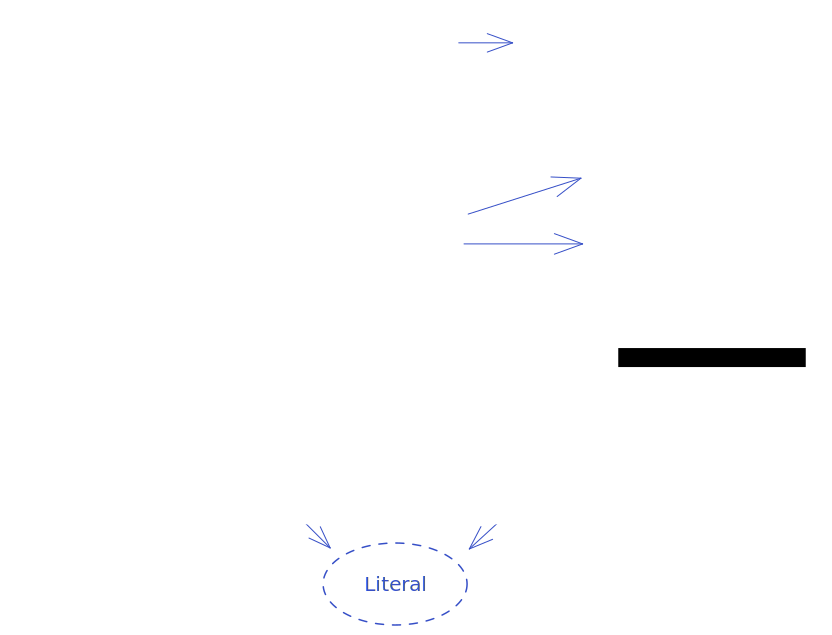
\includegraphics[width=0.8\textwidth]{figures/pdf/omg1.pdf}
        \caption{omg1}
        \label{fig:omg1}
    \end{adjustwidth}
\end{figure}


% query by distance, instance instead adjacent

\begin{listing}[H]
    \inputminted{sparql}{dynamicQueries/inSitu/query.rq}
    \vspace{-0.7cm}
    \caption{Dynamic culling query using GeoSPARQL}
    \label{lst:GeoSPARQLauto}
\end{listing}


\section{In viewer "bot:Space" identification}
% - 1 database + 1 3D enabled instance (viewer) 
%   => viewer can raytrace identify wright space (little computation)
% - 2 layered viewer visible elements / invisible spaces
% - sequence diagram
%   - manual first step + adjacent spaces
%   - all spaces
%   - combination of spaces
% - sample queries

\begin{listing}[H]
    \inputminted{sparql}{dynamicQueries/inViewer/query.rq}
    \vspace{-0.7cm}
    \caption{Querying in viewer "bot:Space" identification}
    \label{lst:BOTauto}
\end{listing}


\section{In query OBJ geometry filtering}
% - no geometric but string analysis in query
% - AABBox filtering of for example obj rooms
% - all negative points

\begin{listing}[H]
    \inputminted{sparql}{dynamicQueries/inQuery/query.rq}
    \vspace{-0.7cm}
    \caption{Querying in query OBJ geometry filtering}
    \label{lst:OBJauto}
\end{listing}

\begin{listing}[H]
    \inputminted{js}{dynamicQueries/inQuery/function.js}
    \vspace{-0.7cm}
    \caption{Querying in situ WKT location}
    \label{lst:OBJautoFunction}
\end{listing}


\chapter{Modular Approach} \label{ch:modularApproach}
% - what is a modular approach
% - why is it important
%   - extendability
%   - maintainability
%   - reusability
% - all modules in basic form
%   - always imrpoovements possible
% - access != modules to rest
% - both specific to culling as to LDBIM viewers in general
% - knowledge was mined from prototype
The theoretical model proposed in this thesis is informed by the practical experiences and observations gained through the development of the prototype.

\section{Data fetching}
% - what I mean by that

\subsection{\acs{sparql} fetcher}
% - handles back and forth communication with rdf database
% - authentication

\subsection{Database fetcher}
% - handles back and forth communication with external database
% - authentication

\section{Cache manager}
% - what I mean by that
% - why is it important
%   - performance
%   - data integrity
% - multitidude of possibilities, such as LRU
% - why not others

\subsection{\acs{lru} algorithm}
% - LRU principle
% - develop needs

\section{Query processing}
% - multiple sources

\subsection{Query builder}
% - challenges that come with it
% - abstraction of dynamic queries in algorithms, 

\subsection{Query composer}
% - combination af multiple queries

\section{Interactions} \label{sec:interactions}
% - diagram + explanations

\section{Sequences}

\chapter{Prototype} \label{ch:prototype}

\begin{figure}[H]
    \centering
    
\includegraphics[width=\textwidth]{figures/pdf/interactions_prototype.pdf}
    \caption[Interactions prototype]{Conceptual diagram of the interactions between the moduwithin the prototype, based on Figure \ref{fig:interactionModules}.}
    \label{fig:interactionPrototype}
\end{figure}


\clearpage
\chapter*{List of Acronyms}
\begin{acronym}[JSONP]\itemsep2pt\hypersetup{hidelinks}
  \acro{aec}[AEC]{Architecture, Engineering and Construction}  
  \acro{ar}[AR]{Augmented Reality}
  \acro{ascii}[ASCII]{American Standard Code for Information Interchange}
  \acro{bcf}[BCF]{\acs{bim} Collaboration Format}
  \acro{bcfowl}[bcfOWL]{\acs{bim} Collaboration Format Ontology}
  \acro{bim}[BIM]{Building Information Modelling}
  \acro{bot}[BOT]{Building Topology Ontology}
  \acro{bvh}[BVH]{Bounding Volume Hierarchy}
  \acro{chc}[CHC]{Coherent Hierarchical Culling algorithm}
  \acro{cpu}[CPU]{Central Processing Unit}
  \acro{dc}[DC]{Drop Culling}
  \acro{fog}[FOG]{File Ontology for Geometry formats}
  \acro{gis}[GIS]{Geographic Information System}
  \acro{gltf}[GLTF]{GL Transmission Format}
  \acro{gml}[GML]{Geography Markup Language}
  \acro{gpu}[GPU]{Graphics Processing Unit}
  \acro{hagi}[HAGI]{Hardware Accelerated Geometry Instancing}
  \acro{hhd}[HHD]{Hand Held Device}
  \acro{ifc}[IFC]{Industry Foundation Classes}
  \acro{ifcowl}[ifcOWL]{Industry Foundation Classes Ontology}
  \acro{json}[JSON]{JavaScript Object Notation}
  \acro{lbd-cg}[LBD-CG]{Linked Building Data Community Group}
  \acro{ldbim}[LDBIM]{Linked Data \acs{bim}}
  \acro{lod}[LOD]{Level of Detail}
  \acro{lru}[LRU]{Least Recently Used}
  \acro{mep}[MEP]{Mechanical, Electrical and Plumbing}
  \acro{nohc}[NOHC]{Near Optimal Hierarchical Culling}
  \acro{oc}[OC]{Occlusion Culling}
  \acro{ogc}[OGC]{Open Geospatial Consortium}
  \acro{omg}[OMG]{Ontology for Managing Geometry}
  \acro{owl}[OWL]{Web Ontology Language}
  \acro{ram}[RAM]{Random Access Memory}
  \acro{rdf}[RDF]{Resource Description Framework}
  \acro{rdfs}[RDFS]{Resource Description Framework Schema}
  \acro{sdk}[SDK]{Software Development Kit}
  \acro{sparql}[SPARQL]{SPARQL Protocol and \acs{rdf} Query Language}
  \acro{sql}[SQL]{Structured Query Language}
  \acro{ui}[UI]{User Interface}
  \acro{uml}[UML]{Unified Modelling Language}
  \acro{uri}[URI]{Uniform Resource Identifier}
  \acro{vfc}[VFC]{View Frustum Culling}
  \acro{vram}[VRAM]{Video Random Access Memory}
  \acro{w3c}[W3C]{World Wide Web Consortium}
  \acro{wkt}[WKT]{Well-Known Text}
  \acro{xml}[XML]{Extensible Markup Language}
  \acro{xsd}[XSD]{\ac{xml} Schema Definition}
\end{acronym}

\printbibliography[nottype=web_page, heading=bibintoc,title={References}]
\printbibliography[type=web_page, heading=bibintoc, title={Referenced webistes}]


\appendix
\chapter{Setup}
\usemintedstyle{default}
% \section{Participants}
% \begin{figure}[h]
%     \centering
%     \includegraphics[width=6cm]{./figures/sequenceDiagram.png}
%     \caption{Sequence diagram}
%     \label{fig:sequendeDiagram}
% \end{figure}
% \section{Framework}
% \subsection{Nextjs}
% \section{Querying}
% \subsection{Front-end}
% \subsection{Back-end}
% \section{Rendering}
% \subsection{Xeokit \acs{sdk}}

\section {Pages}
\subsection{index}
\inputminted{tsx}{figures/snippets/src/pages/index.tsx}
\begin{minted}{tsx}
import dynamic from "next/dynamic";
import Head from "next/head";
import { Navbar, Querypannel } from "~/components";

const ARViewer = dynamic(() => import("~/components/ARViewer"), {
  ssr: false,
});

export default function Home() {
  return (
    <>
      <Head>
        <title>Create T3 App</title>
        <meta name="description" content="Generated by create-t3-app" />
        <link rel="icon" href="/favicon.ico" />
      </Head>
      <main>
        <div className="absolute top-14 h-[calc(100vh-3.5rem)] w-full overflow-hidden">
          <ARViewer />
        </div>
        <Navbar />
        <Querypannel/>
      </main>
    </>
  );
}
\end{minted}
\newpage
\section {Components}
\subsection{ARViewer}
\inputminted{tsx}{figures/snippets/src/components/ARViewer.tsx}
\newpage
\subsection{Navbar}
\inputminted{tsx}{figures/snippets/src/components/Navbar.tsx}
\newpage
\subsection{QueryPannel}
\inputminted{tsx}{figures/snippets/src/components/QueryPannel.tsx}

\newpage
\section {Modules}
\subsection{Viewer}
\subsubsection{useInitViewer}
\inputminted{ts}{figures/snippets/src/modules/viewer/useInitViewer.ts}
\newpage
\subsubsection{useLoadGeometry}
\inputminted{ts}{figures/snippets/src/modules/viewer/useLoadGeometry.ts}
\newpage
\subsection{fetchSPARQL}
\inputminted{ts}{figures/snippets/src/modules/fetchSPARQL.ts}
\newpage
\subsection{useCacheManagement}
\inputminted{ts}{figures/snippets/src/modules/useCacheManagement.ts}

The Xeokit \ac{sdk} ...

\end{document}
